\documentclass[openany]{book}
\usepackage{ctex}
\usepackage{graphicx}
\graphicspath{{../visualize/}{visualize/}}
\usepackage{listings}
\usepackage{xcolor}
\usepackage{geometry}
\usepackage{float}
\geometry{a4paper, margin=2.2cm}

% ===== 代码列表的统一样式 =====
\lstset{
    basicstyle=\ttfamily\scriptsize,
    keywordstyle=\color{blue!80!black},
    commentstyle=\color{green!45!black},
    frame=single,
    rulecolor=\color{gray!60},
    framesep=3pt,
    aboveskip=5pt,
    belowskip=5pt,
    breaklines=true,
    columns=flexible,
    numbers=left,
    numberstyle=\tiny\color{gray},
    showstringspaces=false,
    tabsize=4,
    language=Verilog,
    captionpos=b,
}

\title{不同搜索树的比较}

\begin{document}
\maketitle

\chapter{引言}
\section{实验目的}
树形结构，是计算机科学中最常用的数据结构之一。
它们在数据库、文件系统、编译器等领域都有广泛的应用。
不同的树结构在不同的应用场景下有不同的性能表现。
本实验旨在实现并比较几种常见的搜索树，包括二叉搜索树（BST）、AVL树、红黑树（RBT）、伸展树（Splay Tree）和B+树（BPT），
以了解它们在插入、删除操作上的性能差异。

\section{实验环境}

\begin{itemize}
    \item 编程语言：C
    \item 编译器：gcc
    \item 在算法实现上，我们都使用了迭代的方式，以尽可能控制变量。
\end{itemize}

\chapter{数据结构\&算法描述}
本实验当中用到的数据结构有：
\begin{itemize}
    \item 二叉搜索树(BST)
    \item AVL
    \item 红黑树(RBT)
    \item 伸展树(Splay Tree)
    \item B+树(BPT)
\end{itemize}

我们将会依次描述其实现方式，给出相应算法的描述（伪代码）。

\section{二叉搜索树}
BST 维护左子树键值小于根、右子树键值大于根的性质。
普通 BST 不主动调整树高，有序插入时可能退化为高度为 $N$ 的链。
删除时通过额外指针记录当前结点的父结点，无需使用栈，额外空间复杂度为 $O(1)$。

插入
\begin{lstlisting}
function insertBST(T,key)
    current = T

    if (current == NULL)
        return newNode(key)

    while (True)
        if (key < current->data)
            if (current->left == NULL)
                current->left = newNode(key)
                break
            current = current->left
            
        else if (key > current->data)
            if (current->left == NULL)
                current->left = newNode(key)
                break
            current = current->left
        
        else 
            break

    

\end{lstlisting}

删除
\begin{lstlisting}
function deletionBST(T,key)
    parent = NULL
    current = T

    if (T == NULL)
        return T

    while (current != NULL and current->val != key)
        parent = current
        if (key < current->val)
            current = current->left
        else
            current = current->right

    if (current == NULL)
        return T

    if (current has two non-NULL children)
        successorParent = current
        successor = current->right
        while (successor->left != NULL)
            successorParent = successor
            successor = successor->left
        current->val = successor->val
        parent = successorParent
        current = successor

    child = the non-NULL child of current, if any
    if (parent == NULL)
        T = child
    else if (parent->left == current)
        parent->left = child
    else
        parent->right = child

    free(current)
    return T
\end{lstlisting}

\section{AVL}
AVL使用平衡因子(balance factor)，来维持树的平衡。
记树T的高度为$H_T$，空树高度为-1。
每个结点的平衡因子$bf=H_{T->left}-H_{T->right}$。
对于一棵AVL树，其每个节点的左右子树的高度差小于等于1，
即$bf \in \{-1,0,1\}$。
对树的插入删除都可能会破坏这一性质，
因此，我们需要旋转这种操作来维护这种性质。

\subsection{旋转}
旋转，分为左旋和右旋两种操作，由于两者是镜面对称的，因此我们在这里以左旋为例。
\begin{lstlisting}
function LeftRotate(root)
    pivot = root->right
    root->right = pivot->left
    pivot->left = root

    Update the height and balance factor of root and pivot
    return pivot
\end{lstlisting}

右旋与左旋对称；旋转后返回新的子树根。
旋转操作在接下来几种二叉树当中均会使用，后续就不再赘述了。

\subsection{插入}
先根据BST的插入方式找到插入位置，然后将新结点插入到该位置。
插入后如果破坏了AVL树的性质，则需要进行旋转操作来恢复平衡。
\begin{lstlisting}
function AVLInsert(node, key)
    path = empty stack
    current = node

    Search for the insertion position as in a binary search tree
    and push the node passing by onto the stack

    child = CreateNode(key)
    while (path is not empty)
        current = Pop path
        Attach child to current on the side containing key
        Update the height and balance factor of current

        if (current is unbalanced)
            if (left subtree is higher)
                if (key > current->left->key)
                    current->left = LeftRotate(current->left)
                child = RightRotate(current)
            else
                if (key < current->right->key)
                    current->right = RightRotate(current->right)
                child = LeftRotate(current)
        else
            child = current

    return child
\end{lstlisting}

\subsection{删除}
类似的，先根据BST的删除方式找到删除位置，然后将该结点删除。
相较于插入，删除之后可能需要更多次的旋转以维持平衡。
\begin{lstlisting}
function AVLDelete(node, key)
    path = empty stack
    current = node

    Search for the deletion position as in a binary search tree
    and push the node passing by onto the stack

    if (current == NULL)
        return node

    if (current has two children)
        Push current and the right-child direction onto path
        successor = current->right
        while (successor->left != NULL)
            Push successor and the left-child direction onto path
            successor = successor->left
        current->key = successor->key
        child = successor->right
        Free successor
    else
        child = current's non-NULL child, if any
        Free current

    while (path is not empty)
        (current, direction) = Pop path
        Attach child to current in direction
        Update the height and balance factor of current

        if (current is unbalanced)
            if (left subtree is higher)
                if (current->left balance factor < 0)
                    current->left = LeftRotate(current->left)
                child = RightRotate(current)
            else
                if (current->right balance factor > 0)
                    current->right = RightRotate(current->right)
                child = LeftRotate(current)
        else
            child = current

    return child
\end{lstlisting}

\section{红黑树}
红黑树对每个结点标记颜色（红/黑），其中结点的颜色需满足以下几条性质：
\begin{itemize}
    \item 根的颜色为黑色。
    \item 不能出现连续两个红色结点。
    \item 每条分路（从根到空结点）的黑色结点数相同。
    \item 空结点视为黑色。
\end{itemize}

这个性质保证了最长路径（红黑交替）不超过最短路径（全黑）的两倍。

\subsection{插入}
这里，我们在每个结点当中保存了其父结点的地址，方便回溯、调整。
\begin{lstlisting}
function RBTInsert(T, key)
    Search for the insertion position as in a binary search tree
    If key already exists, return T
    Create a red node new and attach it to its parent
    If new is the root, color it black and return new
    while (new is not the root and its parent is red)
        parent = new->parent
        grandparent = parent->parent
        uncle = the other child of grandparent

        if (uncle is red)
            Color parent and uncle black, and grandparent red
            new = grandparent
        else
            if (parent is the left child of grandparent)
                if (new is the right child of parent)
                    new = parent
                    LeftRotate(parent)
                Color new's parent black and grandparent red
                RightRotate(grandparent)
            else
                if (new is the left child of parent)
                    new = parent
                    RightRotate(parent)
                Color new's parent black and grandparent red
                LeftRotate(grandparent)
            Stop adjusting

    Follow parent pointers to the root and color it black
    return T
\end{lstlisting}

\subsection{删除}
删除时将实际摘除结点的原颜色记录下来。若其为黑色，则通过调整替代结点及其兄弟结点，恢复各条路径的黑高；空结点视为黑色。
\begin{lstlisting}
function RBTDelete(T, key)
    z = Search for key as in a binary search tree
    if (z == NULL)
        return T

    y = z
    xParent = z->parent
    if (z has at most one child)
        x = z's non-NULL child, if any
        originalColor = z->color
        Replace z with x; update T if z is the root
        If x is not NULL, update x->parent
    else
        y = findmin(z->right)
        originalColor = y->color
        x = y->right
        if (y->parent == z)
            xParent = y
            If x is not NULL, set x->parent = y
        else
            xParent = y->parent
            Replace y with x
            y->right = z->right
            y->right->parent = y
        Replace z with y; update T if z is the root
        y->left = z->left
        y->left->parent = y
        y->color = z->color

    Free z

    if (originalColor == BLACK)
        // NULL is black; xParent also tracks x when x is NULL
        while (x != T and x is black)
            if (xParent == NULL)
                break
            if (x is the left child of xParent)
                w = xParent->right
            else
                w = xParent->left

            if (w is red)
                Color w black and xParent red
                if (x is the left child)
                    LeftRotate(xParent)
                else
                    RightRotate(xParent)
                Update T if the root changed
                Reassign w

            if (w == NULL)
                x = xParent
                xParent = x->parent
                Continue
            else if (both children of w are black)
                Color w red
                x = xParent
                xParent = x->parent
            else
                if (x is the left child)
                    if (w->right is black)
                        Color w's left child black and w red
                        RightRotate(w)
                        Reassign w
                    Give w xParent's color; color xParent and w's right child black
                    LeftRotate(xParent); update T if the root changed
                else
                    if (w->left is black)
                        Color w's right child black and w red
                        LeftRotate(w)
                        Reassign w
                    Give w xParent's color; color xParent and w's left child black
                    RightRotate(xParent); update T if the root changed
                x = T
                Stop adjusting

    If x is not NULL, color it black
    If T is not NULL, follow parent pointers to the root
    return T
\end{lstlisting}

\section{伸展树}
Splay Tree 在每次访问后将目标节点（或最后访问节点）伸展到根，
单次最坏复杂度为 $O(N)$，但任意序列的摊还复杂度为 $O(\log N)$。

在这里，Splay 使用 top-down 算法。临时头结点把访问路径拆为左、中、右三部分，循环执行 zig-zig 和链接，最后重新拼接。
插入先伸展目标键，再把新节点置于根；删除先伸展目标，若存在则将左子树最大节点伸展到根并接回原右子树。
这样不需要保留父节点信息，也不需要使用显式栈。

top-down算法当中，重要操作就是splay
\begin{lstlisting}
function splay(T, key)
    if (T == NULL)
        return NULL

    header.left = NULL
    header.right = NULL
    leftTree = header
    rightTree = header
    root = T

    while (True)
        if (key < root->val)
            if (root->left == NULL)
                break
            if (key < root->left->val)
                root = RightRotate(root)
                if (root->left == NULL)
                    break
            rightTree->left = root
            rightTree = root
            root = root->left
        else if (key > root->val)
            if (root->right == NULL)
                break
            if (key > root->right->val)
                root = LeftRotate(root)
                if (root->right == NULL)
                    break
            leftTree->right = root
            leftTree = root
            root = root->right
        else
            break

    leftTree->right = root->left
    rightTree->left = root->right
    root->left = header.right
    root->right = header.left
    return root

\end{lstlisting}

插入
\begin{lstlisting}
function insertSplay(T, key)
    if (T == NULL)
        return newNode(key)

    T = splay(T, key)
    if (T->val == key)
        return T

    node = newNode(key)

    if (key < T->val)
        node->left = T->left
        node->right = T
        T->left = NULL
    else
        node->right = T->right
        node->left = T
        T->right = NULL

    return node
\end{lstlisting}

删除
\begin{lstlisting}
function delete(root, key):
    if (root == NULL)
        return NULL

    root = splay(root, key)

    if (root.key != key)              // 不存在
        return root

    if (root.left == NULL)
        newRoot = root.right
    else
        newRoot = splay(root.left, key)   // key 在左子树中最大
        newRoot.right = root.right        // 此时 newRoot.right 必为 NULL
    return newRoot
\end{lstlisting}

\section{B+树}
与其他的树不同的是，B+树是一种多叉的搜索树，
所有的数据存储在叶子结点上，每个叶子结点的高度相同，同时其叶子结点之间通过链表相连，方便范围查询。
其多叉的性质使得B+树在磁盘存储上有更好的性能，可以显著减少磁盘I/O次数。
对于一棵order为M的B+树，其每个结点最多有M个子结点，至少有$\lceil M/2 \rceil$个子结点。
在实现方式上，我们使用结点的数组来存储其子结点的指针，同时使用一个数组来存储其关键字。

数据结构体定义如下：
\begin{lstlisting}
typedef struct Bn
{
    int leaf; //判断是否为叶节点，便于分配链表指针
    int* data; //关键字数组
    int num; //当前关键字个数

    struct Bn** children; //子结点指针数组
    struct Bn* next; //叶子结点的链表指针，指向下一个叶子结点
    struct Bn* prev; //叶子结点的链表指针，指向上一个叶子结点
}BNode;
\end{lstlisting}

插入
\begin{lstlisting}
//树order为M
function insertBPT(T,key)
    path = empty stack
    Search for the insertion position as in a search tree
    and push the node passing by onto the stack

    I = key
    C1 = NULL
    C2 = NULL
    while (True)
        if (path is empty)
            root = newNode()
            root->data[0] = I
            root->children[0] = C1
            root->children[1] = C2
            if (C1 != NULL && C2 != NULL)
                root->leaf = true
            l=else
                root->leaf = false
            T = root
            break

        current = Pop path

        insert I into current's data array

        if (C1 != NULL && C2 !=NULL)
            insert C1&C2 into current's children array in the corresponding position

        if (current->num > M)
            split current into two node: A & B

            if (current is leaf)     
                A->next = B 
                B->prev = A 
                if (current->prev != NULL)
                    current->prev->next = A 
                else 
                    update the ptr pointing to the head of the linked list
                B->next = current->next

            free(current)

            I = the first key of B 
            C1 = A
            C2 = B

        else
            break

    return T
\end{lstlisting}

删除
\begin{lstlisting}
function deleteBPT(T,key)
    if (T->root == NULL)
        return NULL

    path = empty stack
    current = T->root
    while (current is not a leaf)
        Find childIndex such that key belongs to current->children[childIndex]
        Push (current, childIndex) onto path
        current = current->children[childIndex]

    Find key in current->data
    if (key is not found)
        return T

    Remove key from current->data and decrease current->num
    if (the deleted key was the first key and current->num > 0)
        Update the affected separator key in its ancestors

    minKeys = floor(T->order / 2)
    while (current is not the root and current->num < minKeys)
        (parent, childIndex) = Pop path
        left = parent->children[childIndex - 1], if childIndex > 0
        right = parent->children[childIndex + 1], if childIndex < parent->num

        if (current is a leaf)
            if (left/right exist and have at least minKeys)
                Move left's/right's largest/smallest key to the front of current->data
                Update parent->data
                Update affected ancestor separators if the subtree minimum changed
                break
            else if (left/right exist but have less than minKeys)
                merge current and left/right
                update linked list pointers
                update parent->data and parent->children   
                Free current
            
        else
            if (left/right exist and have at least minKeys)
                Move parent->data[childIndex - 1]/[childIndex] to the front/end of current->data
                Move left's/right's last/first child to the front/end of current->children
                Move left's/right's largest/first key up to parent->data[childIndex - 1]/[childIndex]
                break
            else if (left/right exist but have less than minKeys)
                merge current and left/right
                Remove parent->data[childIndex - 1]/[childIndex] and parent->children[childIndex]/[childIndex + 1]
                Free current

        current = parent

    if (T->root is an internal node and T->root->num == 0)
        oldRoot = T->root
        T->root = oldRoot->children[0]
        Free oldRoot

    if (T->root is a leaf and T->root->num == 0)
        Free T->root
        T->root = NULL
        T->head = NULL
        return T

    T->head = the leftmost leaf under T->root
    return T
\end{lstlisting}

\chapter{实验结果}
我们将实验当中各个树用时与数据量的关系作图，分为线性坐标轴与对数坐标轴。
图表当中的用时是摊还用时，即若干次操作的总用时除以操作的数量。

\begin{figure}[H]
    \centering
    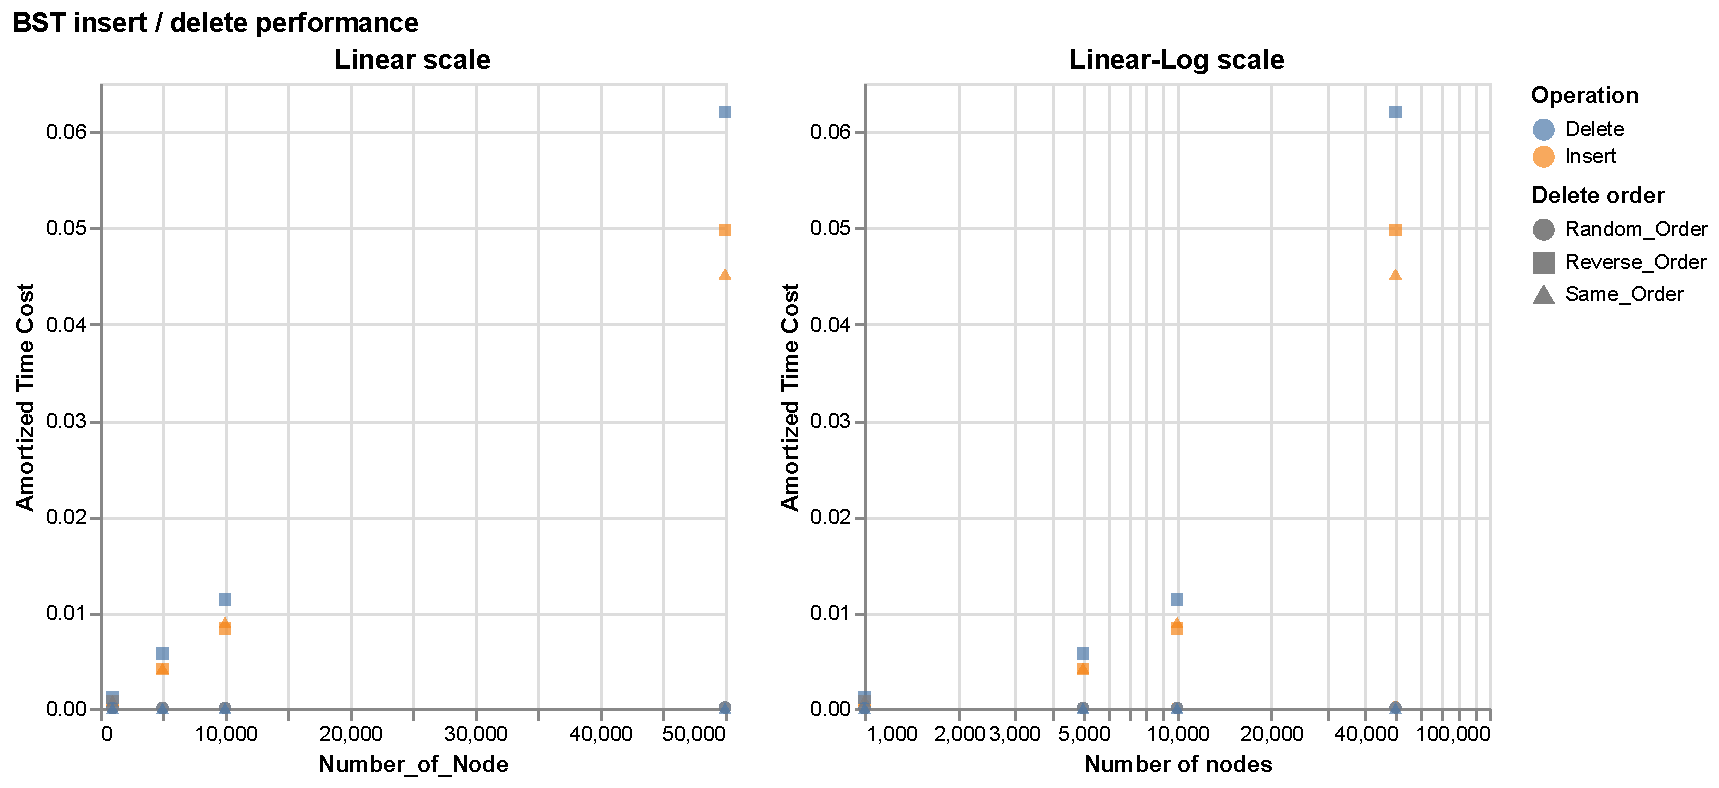
\includegraphics[width=0.7\textwidth]{BST_combined.pdf}
    \caption{BST实验结果}
    \label{fig:bst_results}
\end{figure}
对于普通BST，当插入数据是有序时，树会退化为链表。
此时如果按插入顺序删除，每次删除的结点正好在根，这使得删除只需要消耗$O(1)$的时间。
而若是按逆序删除，则每次删除的结点都在叶子结点，删除需要消耗$O(N)$的时间。
实验当中顺序删除的用时几乎为零，而逆序删除的用时呈现线性增长。且耗时远大于接下来的几种平衡二叉树。

\begin{figure}[H]
    \centering
    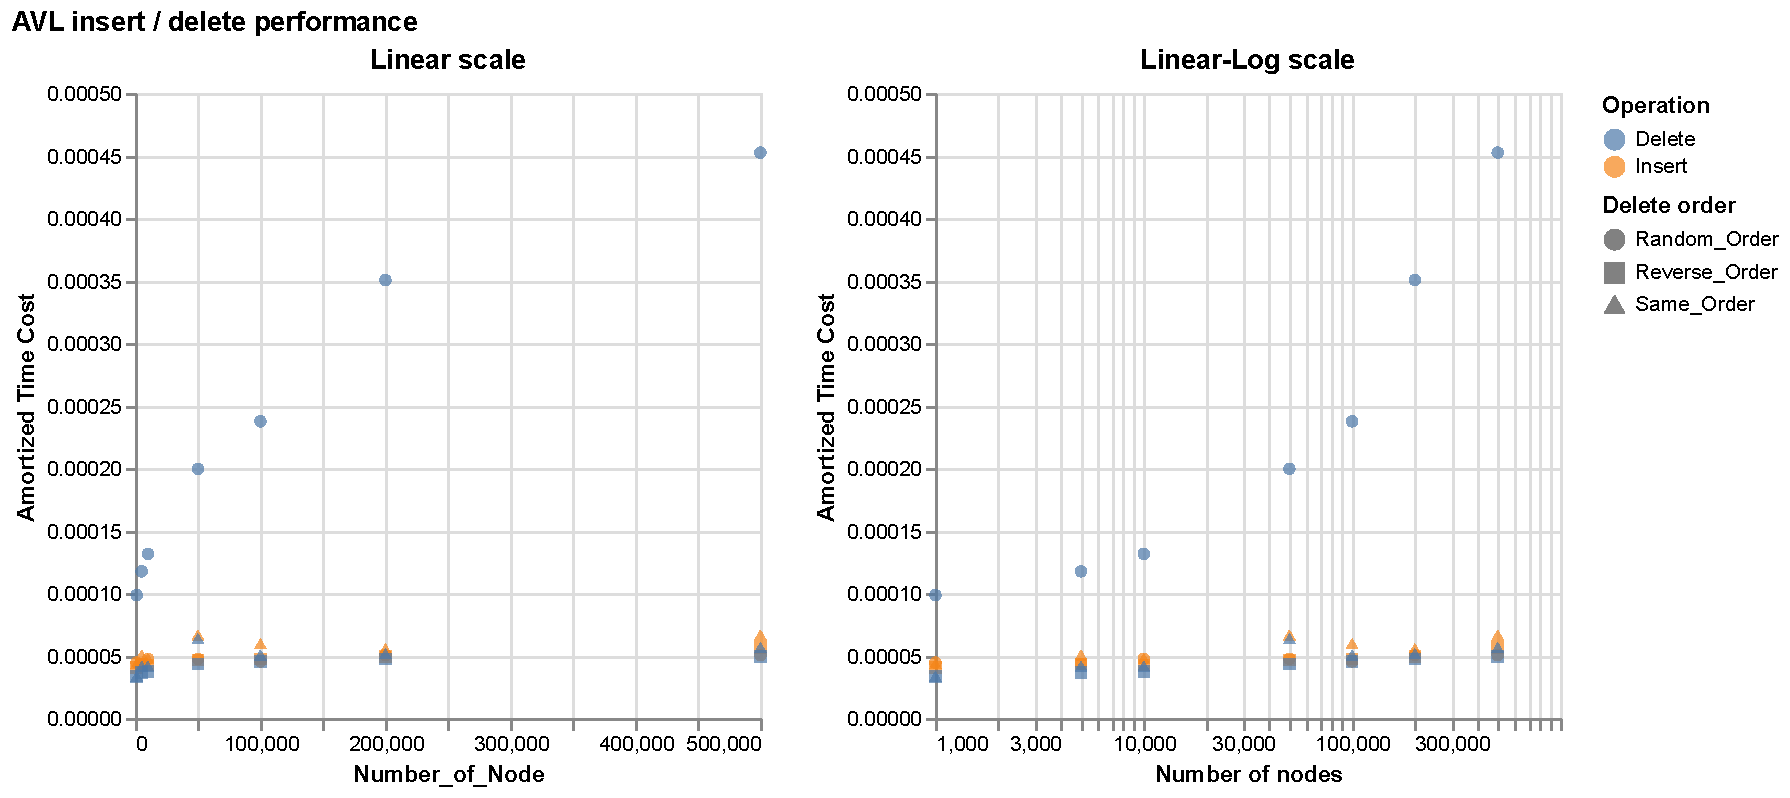
\includegraphics[width=0.7\textwidth]{AVL_combined.pdf}
    \caption{AVL实验结果}
    \label{fig:avl_results}
\end{figure}

\begin{figure}[H]
    \centering
    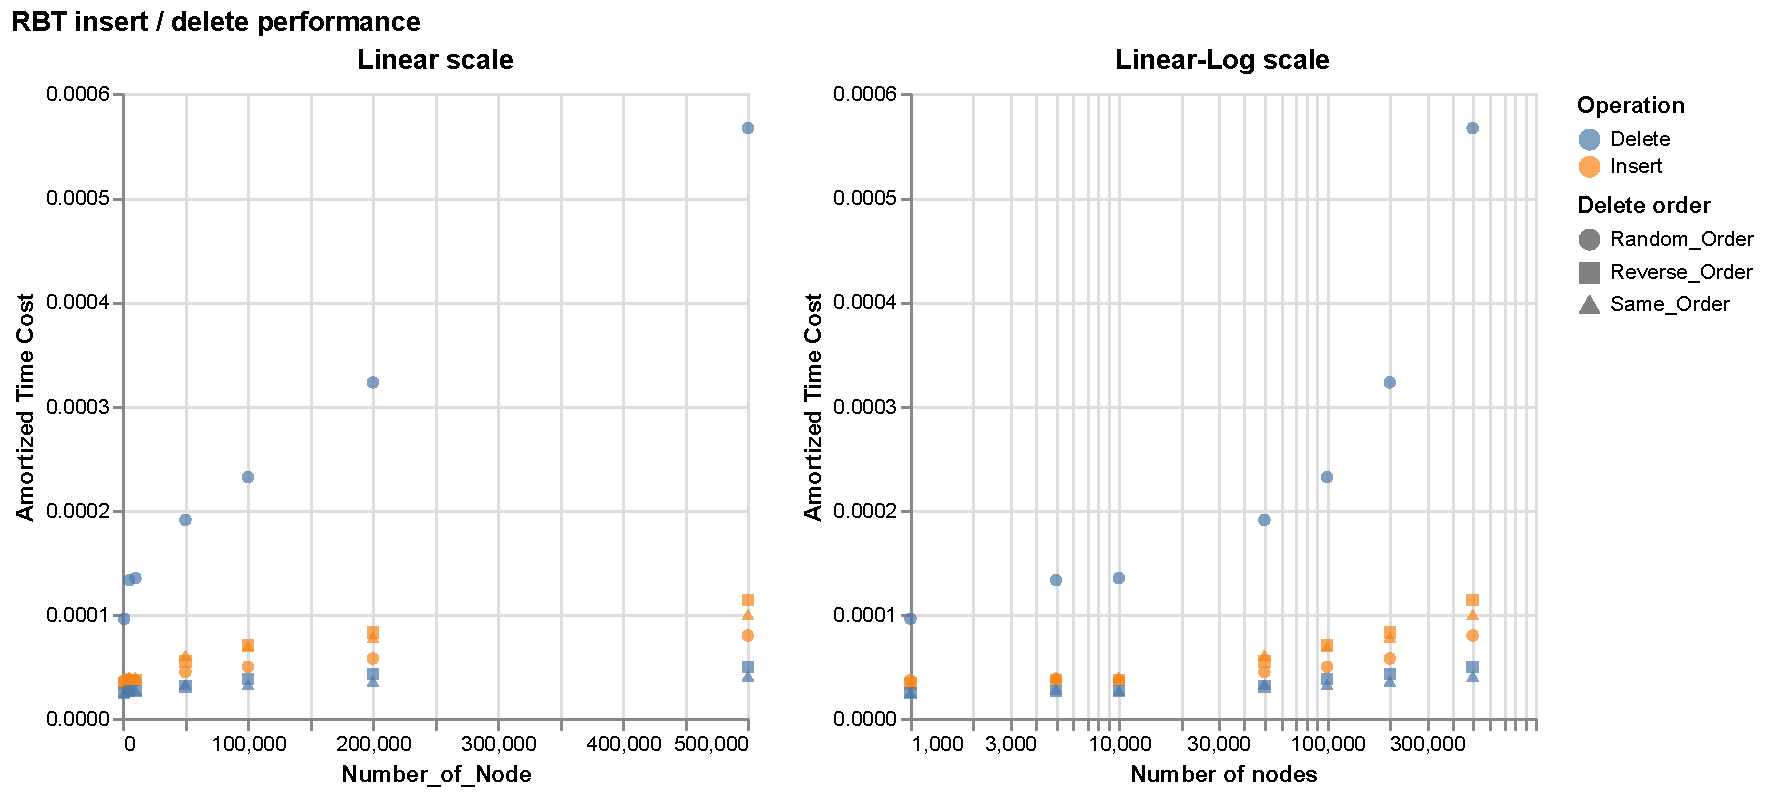
\includegraphics[width=0.7\textwidth]{RBT_combined.pdf}
    \caption{RBT实验结果}
    \label{fig:rbt_results}
\end{figure}

AVL和RBT都是平衡二叉树，插入和删除的时间复杂度均为$O(\log N)$。
这点在实验结果中得到了验证，随着数据量的增加，AVL和RBT的用时呈现对数增长。
但是AVL的平衡相较于RBT的平衡更加严格，因此AVL的插入和删除操作需要更多的旋转操作，导致其用时略高于RBT。
这点在我们的实验图像当中得到了体现，AVL的曲线在RBT曲线之上。
这说明RBT在综合性能上优于AVL，尤其是在插入和删除操作频繁的场景下。

\begin{figure}[H]
    \centering
    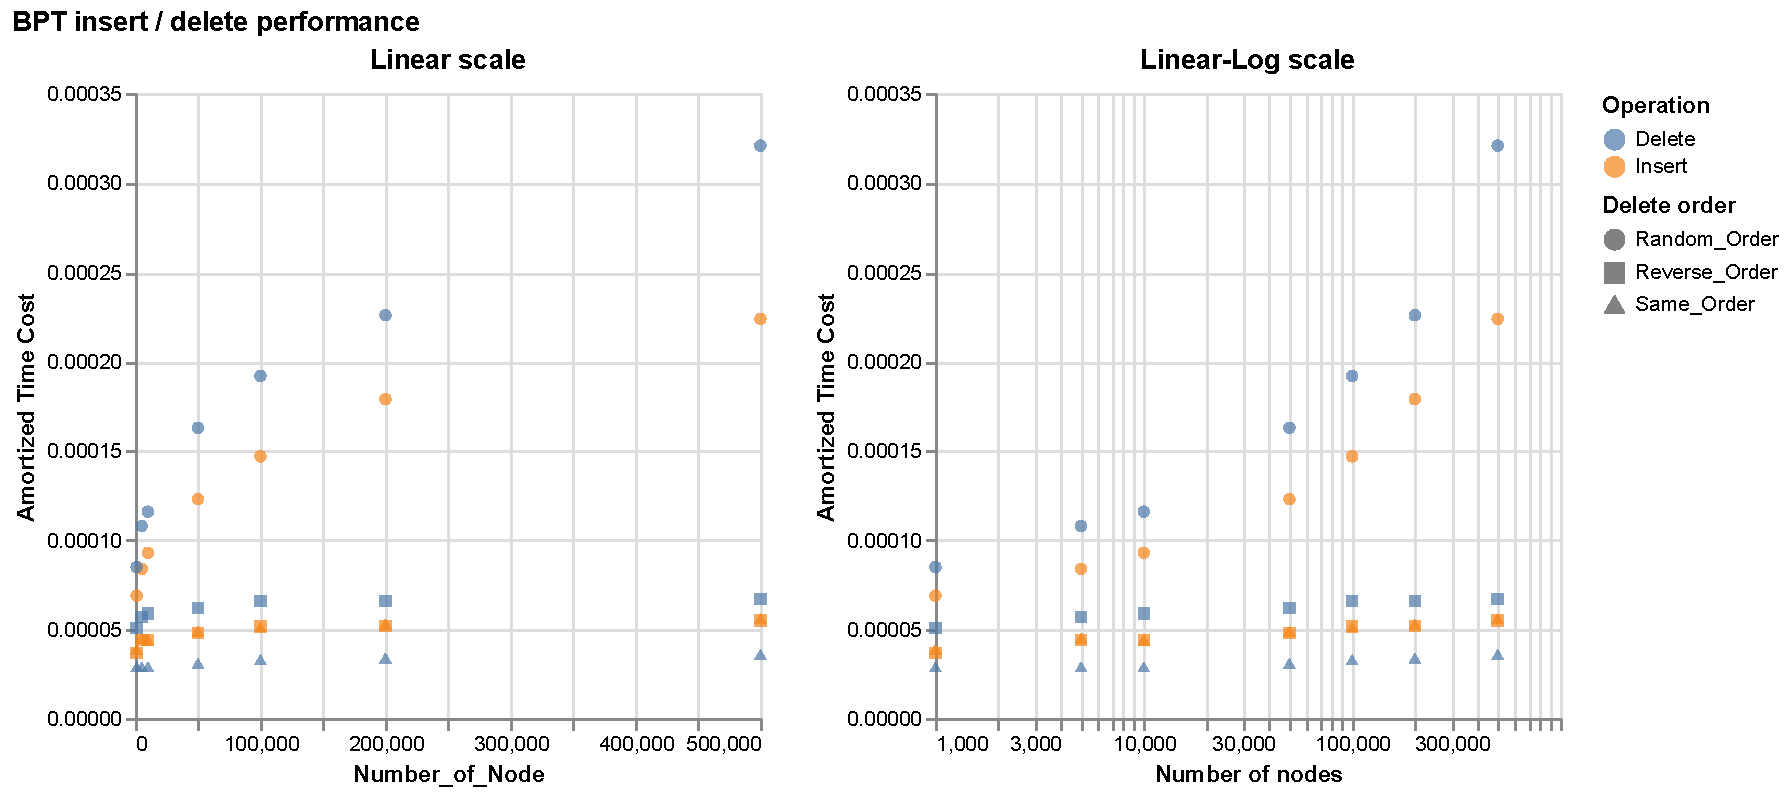
\includegraphics[width=0.7\textwidth]{BPT_combined.pdf}
    \caption{BPT实验结果}
    \label{fig:bpt_results}
\end{figure}

BPT是一种多叉平衡树，适用于磁盘存储和大数据量的场景。
由于BPT的多叉性质，它在插入和删除操作中需要进行更多的节点分裂和合并操作，这使得其在小数据量下的性能不如AVL和RBT。
然而，随着数据量的增加，BPT的性能优势逐渐显现出来，尤其是在大数据量下，BPT的用时明显低于AVL和RBT。

\begin{figure}[H]
    \centering
    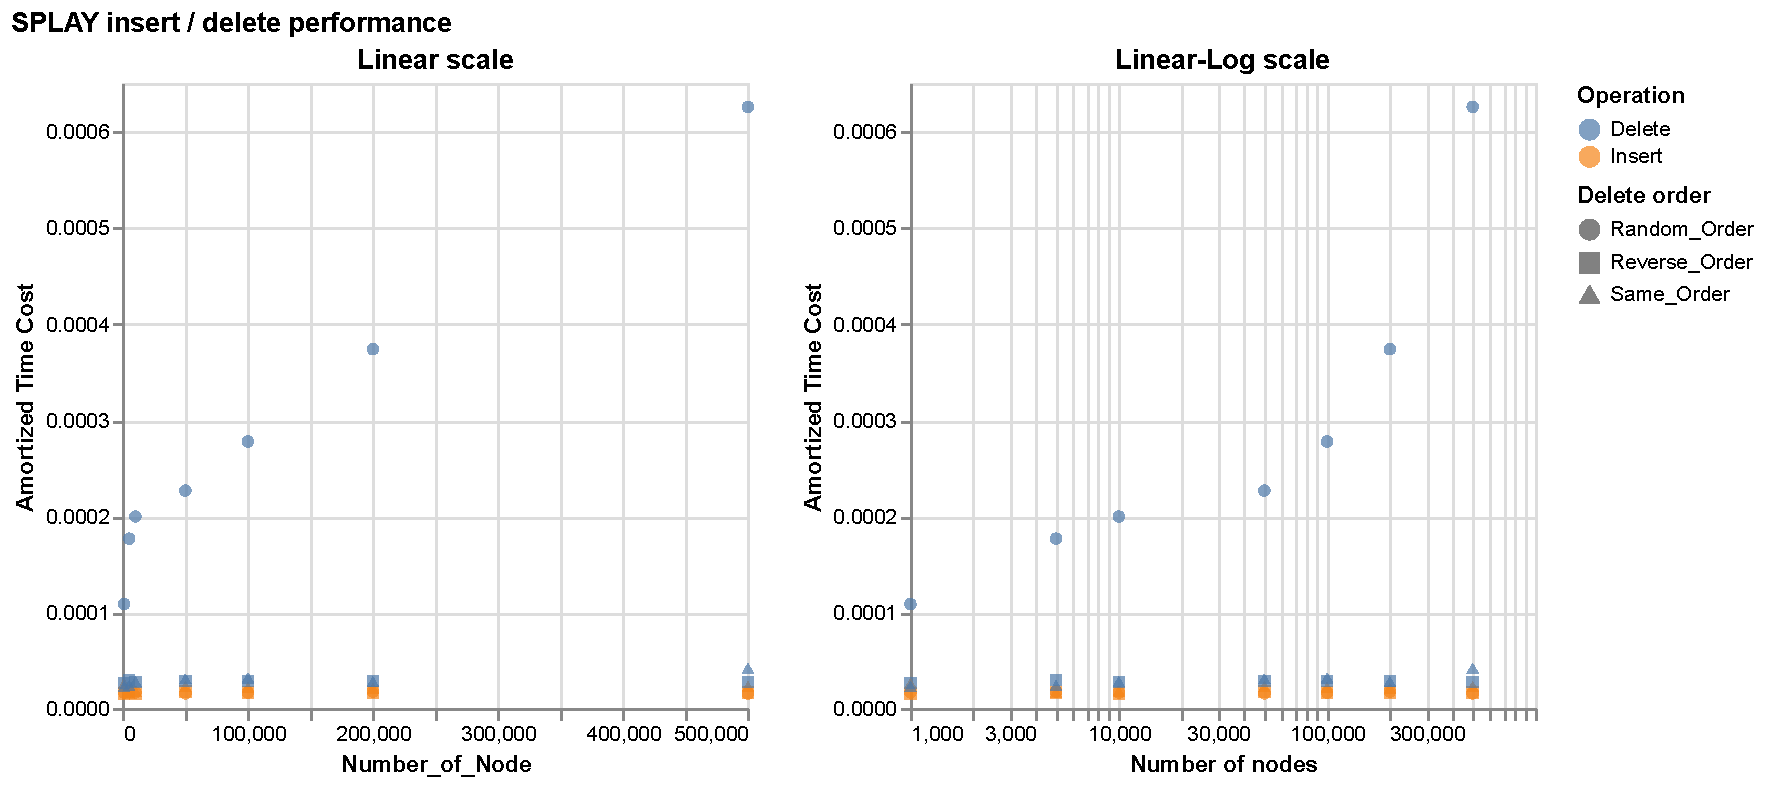
\includegraphics[width=0.7\textwidth]{SPLAY_combined.pdf}
    \caption{SPLAY实验结果}
    \label{fig:splay_results}
\end{figure}
Splay Tree在每次访问后将目标节点伸展到根，这使得它在访问局部性较强的场景下表现出色。
在我们的实验中，Splay Tree的用时在有序插入和删除的情况下表现优异，尤其是在顺序删除的场景下，其用时几乎为常数。

\chapter{总结}
本次实验，我们实现了五种常见的搜索树，并对它们在插入和删除操作上的性能进行了比较。
实验结果表明：
\begin{itemize}
    \item 普通BST在有序数据下会退化为链表，导致插入和删除操作的性能大幅下降。
    \item AVL和RBT作为平衡二叉树，能够保持较好的性能，其中RBT在综合性能上优于AVL。
    \item BPT在大数据量下表现出色，适用于磁盘存储和大数据量的场景。
    \item Splay Tree在访问局部性较强的场景下表现优异，尤其是在顺序删除的情况下，其用时几乎为常数。
\end{itemize}
综上所述，选择合适的搜索树结构对于不同的应用场景至关重要。在实际应用中，应根据数据的特点和操作的频率来选择最适合的搜索树，以获得最佳的性能表现。
\end{document}